\documentclass[11pt,a4paper]{article}

\usepackage[T1]{fontenc}
\usepackage[utf8]{inputenc}
\usepackage{amsmath}
\usepackage{booktabs}
\usepackage{array}
\usepackage{geometry}
\usepackage{graphicx}
\usepackage{hyperref}
\usepackage{lmodern}
\usepackage{microtype}
\usepackage{natbib}
\usepackage{parskip}

\geometry{margin=1in}
\graphicspath{{../figures/}{../artifacts/report_inputs/}}
\newcolumntype{L}[1]{>{\raggedright\arraybackslash}p{#1}}
\bibliographystyle{plainnat}
\hypersetup{
  colorlinks=true,
  linkcolor=black,
  citecolor=black,
  urlcolor=blue,
  pdftitle={From Refining Capacity to Import Dependence: Portugal's Diesel and Gasoline Market, 1990--2024},
  pdfauthor={Diogo Ribeiro}
}

\title{From Refining Capacity to Import Dependence:\\
Portugal's Diesel and Gasoline Market, 1990--2024}
\author{Diogo Ribeiro\thanks{School of Media Arts and Design, Polytechnic of Porto.
ORCID 0009-0001-2022-7072.}}
\date{2026-08-21}

\begin{document}

\maketitle

\begin{abstract}
\noindent
Portugal's refining system gained diesel conversion capability when the Sines hydrocracker
entered commercial production in 2013, and lost one of its two refineries when refining ceased
at Matosinhos in May 2021. Using Eurostat annual oil balances for Portugal and Spain, JODI
monthly physical flows, DGEG national statistics and the European Commission Weekly Oil
Bulletin, this paper measures how the product balance and price exposure changed over
1990--2024.

Portuguese demand dieselised as it did across Europe, and for the same fiscal reason
\citep{harding2014diesel, silva2022different}: the continent's refineries were left over-producing
gasoline and under-producing diesel \citep{deboncourt2013refining}. Against that
background, Portugal's diesel trade position crosses the same line three times: a net exporter
through most of the 1990s, a net importer for the fourteen years from 1999, an exporter again
from 2013 in every year but 2019, and an importer in every year since 2021. The 2013
hydrocracker therefore restored a position the country had held before, and the 2021 closure
carried the system past the dependence it had run in the 2000s. By 2023 domestic manufacturing
covers $0.678$ of diesel demand and the net-import-to-demand ratio reaches $0.262$, which is the
dependence Portugal ran in 2009--2011 on half the manufacturing base it had then. Gasoline,
which entered each event with output far above domestic demand, moves as far on both ratios but
crosses neither threshold. On prices, both Portugal--Spain pairs are cointegrated in log levels
and the diesel error-correction speed increases several-fold after May 2021. The gasoline
change does not survive allowing the long-run relation to shift at its estimated 2013 break.

No causal effect is claimed. The closure and the March 2022 European supply shock fall ten
months apart, and no design here separates their contributions.
\end{abstract}

\vspace{1em}
\noindent\textbf{Keywords:} refining capacity; import dependence; petroleum products; energy
security; price co-movement; Portugal

\section{Introduction}
\label{sec:intro}

Portugal operated two refineries for most of the period studied here. Sines, the larger,
received a hydrocracker that entered commercial production in January 2013 and was intended to
raise diesel yield relative to fuel oil \citep{galphydrocracker}. Matosinhos ceased refining in
May 2021 following a December 2020 announcement, concentrating Portuguese refining at Sines
\citep{galpmatosinhos}. Ten months later, in March 2022, the withdrawal from Russian oil
products disturbed European product supply generally, and vacuum gas oil, a diesel feedstock at
Sines, in particular \citep{galprussian}.

This paper asks whether the loss of refining capacity increased Portugal's dependence on
imported finished petroleum products, and whether Portugal--Spain price co-movement changed
after the closure. I answer both descriptively and by association, not causally, for reasons set
out in Section~\ref{sec:discussion}.

The answer is a sequence of events, and the sequence is the argument. Portugal was a net diesel
exporter through most of the 1990s, in eight of the nine years from 1990. It crossed into net
import at the end of that decade and stayed there for fourteen consecutive years. In 2013 the
hydrocracker shifts the product slate towards middle distillates and Portugal crosses back into
net export, holding that position in every year from 2013 to 2018, with 2019 a single-year
interruption and 2020 a brief return. In May 2021 Matosinhos closes and the crossing reverses a
third time. Every year since has been a net-import year, and in 2023 the net-import-to-demand
ratio reaches $0.262$, the highest in the window, while domestic manufacturing covers $0.678$ of
diesel demand, the lowest.

Read this way the three breaks are not unrelated events but one system crossing and re-crossing
a single line. That framing matters for what the 2013 unit did, which was not to move
Portugal somewhere new but to restore a trade position the country had held in the early
1990s. And it
matters for what followed, because the 2021 closure did not merely undo that restoration. It
carried the system past the dependence it had run in the 2000s, to the most import-dependent
year in thirty-five.

Three features distinguish the exercise. The annual panel runs from 1990, which is early enough
for the 1990s export position to be visible and therefore for the 2013 unit to be read as a
restoration rather than a novelty. A panel beginning in 2005, as an earlier version of this
analysis did, supports the opposite reading. The monthly design separates the May 2021 closure
from the March 2022 shock, which annual data cannot do with ten months between them. And every
quantity reported here is checked mechanically against a checksummed evidence bundle before
publication, with the checks and their limits described in Section~\ref{sec:verification}.

Section~\ref{sec:setting} describes the setting and the data. Section~\ref{sec:design} defines
what resilience is taken to mean here and states the designs. Section~\ref{sec:results} reports
results. Section~\ref{sec:discussion} interprets them and states what cannot be inferred.

\section{Setting and data}
\label{sec:setting}

Four independent bodies publish the series used here. JODI supplies monthly secondary-product
imports, exports, refinery output and demand, and carries per-observation assessment codes
\citep{jodi}. Eurostat's \texttt{nrg\_cb\_oil} supplies the annual oil balance for Portugal and
Spain on a common definition, and is the only source reaching back to 1990 \citep{eurostat}.
DGEG, the Portuguese national statistical authority, publishes annual product trade workbooks
from 2019 \citep{dgegtrade} and a domestic sales series from 1970 \citep{dgegsales}. The
European Commission Weekly Oil Bulletin supplies weekly consumer prices with and without taxes
from 2005 \citep{oilbulletin}. Galp corporate disclosures supply dated refinery events. They are
used as event metadata only, never as outcome data, and the December 2020 announcement date is
deliberately not treated as the physical closure date.

Each arm therefore runs over the study window intersected with what its own source provides: the
annual balance over 1990--2024, the monthly flows over 2002--2024 at $276$ months per product,
and the weekly prices over 2005--2024 at $993$ modelled weeks. The bulletin skips weeks: of the
$1{,}044$ weeks spanned, $995$ are present for Portugal and $994$ for Spain, and I drop the
gaps, so a differenced observation spanning one is a multi-week change entered as a single week.

Diesel is JODI \texttt{GASDIES} and Eurostat \texttt{O4671}, gas oil and diesel oil. Gasoline is
JODI \texttt{GASOLINE} and Eurostat \texttt{O4652}, motor gasoline. Aviation gasoline is excluded
from both. Differing biofuel treatment does not drive residual differences between sources, since the
Eurostat blended-biofuel wedge is $0.0$~kt on exports in every year of the window and at most
$4.5\%$ on imports.

Coverage within those windows is complete. Eurostat carries all 280 product-flow cells for both
countries from 1990, every JODI year in the window carries twelve observed months, and the price
bulletin supplies 995 Portuguese and 994 Spanish weekly observations per product.

One coverage gap is material. DGEG publishes product trade workbooks only from 2019, so for
earlier years I run the trade cross-check against Eurostat rather than against the DGEG primary
publication. That is weaker corroboration than it appears, because Eurostat's Portuguese oil
data is compiled from the DGEG national submission and tracks it to a median difference of
$0.00\%$ across the 2019--2024 cells where both exist. Eurostat is best understood as a second
channel for the same national statistics, not an independent third opinion. Domestic demand is
unaffected, since the DGEG sales series covers the whole window.

Where two genuinely independent sources disagree, both values are reported. Nine of eighty
JODI--Eurostat cells and eight of twenty-four JODI--DGEG cells diverge beyond tolerance. No
divergent cell enters a headline figure without the alternative value being reported alongside
it, and the one case where this changes a conclusion is marked wherever it appears.

\section{Measurement and design}
\label{sec:design}

\subsection{What resilience is taken to mean}

Energy security has no single accepted measure, and the reviews that map the field note that no
study operationalises all its dimensions at once \citep{kruyt2009indicators,
ang2015energysecurity}. Existing quantitative work concentrates on source diversification,
political risk and transport risk \citep{cohen2011measuring}, and the link between import
diversification and security is contested \citep{vivoda2009diversification}. What follows is
narrower than any of these, and deliberately so: it is the part of the concept a national
product balance and a bilateral price relation can measure.

Resilience here means the capacity of Portugal's domestic refining and its trade channels to
absorb a product-specific supply shock without a sharp increase in import reliance or in
exposure to prices formed elsewhere. The definition is deliberately narrow, and the narrowness is
why it can be tested, because it asks about the observable response of a physical balance and
a price relation rather than about whether supply is secure. Four quantities carry it.

The \emph{domestic supply buffer} is refinery output over domestic demand. This is a capability
measure rather than a self-sufficiency measure, since output may be exported while demand is
met by imports, which is the normal state for Portuguese gasoline. \emph{Import exposure} is measured
both as gross import dependence, imports over demand, and as the net-import-to-demand ratio,
which is negative for a net seller and positive for a net buyer. A system can move on one without
moving on the other, which is what happens around 2000. \emph{Concentration} is how many places
the manufacturing happens in, and Portugal moved from two refineries to one in May 2021.
\emph{Price integration} is how closely and how quickly domestic pre-tax prices track a
neighbouring market's, which is the price-side counterpart of physical exposure.

For fuel $j$ in year $t$, with imports $M$, exports $X$, demand $D$ and refinery output
$Q^{\text{refinery}}$:
\[
\text{GrossImportDependence}_{j,t}=\frac{M_{j,t}}{D_{j,t}},
\qquad
\text{NetImportToDemandRatio}_{j,t}=\frac{M_{j,t}-X_{j,t}}{D_{j,t}},
\]
\[
\text{RefineryOutputToDemandRatio}_{j,t}=\frac{Q^{\text{refinery}}_{j,t}}{D_{j,t}}.
\]

Several things that belong to a full account of security of supply are absent, and their absence
bounds every claim made here. Compulsory stocks and commercial inventory are not observed, and
stockholding is the first line of defence against an interruption. Port, storage and pipeline
capacity are not observed, nor are supplier diversification, crude slate, contractual terms, or
spare capacity at the remaining site. A country importing a large share of its diesel through
deep, well-connected markets may be more secure than one manufacturing more of its own from a
single vulnerable feedstock route, and nothing here distinguishes those cases.

\subsection{Designs}

Annual breaks are tested by Chow tests \citep{chow1960tests} on a linear trend at candidate
break years, of which 2013 and
2022 were pre-specified and 2000 is exploratory, with 2021 excluded as a transition year so that
it is assigned to neither side, and Benjamini--Hochberg adjustment \citep{benjamini1995controlling} across all twenty-four
tests. Because the outcomes are mechanically linked, the dependence-robust Benjamini--Yekutieli
form \citep{benjamini2001control} is reported beside it, and it costs two of the six survivors.

The annual interrupted trends are ordinary least squares with a common trend, a post-event
level term and a post-event slope term, HAC(1) covariance, 2021 again excluded. This retains all
annual observations rather than splitting the series.

Monthly event timing comes from a segmented regression \citep{wagner2002segmented,
bernal2017interrupted} on $276$ monthly observations with month
fixed effects, a calendar-month trend and HAC(3) errors. Each phase-trend interaction is centred
on its phase boundary, so a phase coefficient is the level shift at that boundary measured
against the extrapolated pre-closure trend, and the companion trend term is the change in slope
within the phase. The two must be quoted together, and a phase coefficient is not an increment on
the phase before it.

The retail fuel price literature is largely concerned with asymmetry in how quickly prices
rise and fall \citep{bacon1991rockets, borenstein1997gasoline, peltzman2000prices}, a finding
whose robustness has been questioned \citep{bachmeier2003new} and whose methods have been
surveyed with the warning that the field is technique-driven \citep{meyer2004asymmetric}. No
asymmetry is estimated here. The closest published relative runs its diagnostics on euro-area
consumer fuel prices from the same bulletin before choosing a specification
\citep{meyler2009passthrough}, and testing a long-run coefficient against a value implied in
advance follows \citet{bachmeier2006testing}.

For prices, I select the model family from stationarity and cointegration diagnostics, and run
the diagnostics on log levels because that is the scale the models are estimated on. Testing the
EUR per 1000~litres levels instead answers a question about different series, and the two
disagree where it matters, since diesel Engle--Granger is $0.057$ on the EUR levels and below
$0.001$ on logs. I admit a levels regression only on rejection at one per cent rather than five,
because regressing one near-integrated series on another is the spurious-regression case while
an unnecessary error-correction model still nests the difference specification. Neither product
clears that bar, and both pairs are cointegrated in logs, so both are fitted as two-step Engle--Granger
error-correction models \citep{engle1987cointegration}, estimated with
heteroskedasticity- and autocorrelation-consistent covariance throughout \citep{newey1987simple,
andrews1991heteroskedasticity} and on pre-tax prices as the primary measure.

\section{Results}
\label{sec:results}

\subsection{The physical balance}

Over 1990--2024, Portuguese diesel demand averaged $4{,}522$~kt against average refinery output
of $4{,}348$~kt, average imports of $804$~kt and average exports of $643$~kt. Gasoline output
averaged $2{,}337$~kt against demand of $1{,}511$~kt, a surplus exported at an average of $971$~kt
a year against imports of only $129.5$~kt. Output therefore fell short of demand on average across the
window, and the shortfall was covered by buying more than the country sold. For gasoline the
arithmetic runs the other way and by a wide margin, since the country manufactured more than
it could burn and had to find a buyer for the rest.

That the two products sit in opposite positions relative to the same domestic demand is the
single most important fact for reading what follows. A loss of refining capacity acts on a
deficit in one product and on a surplus in the other, so the same proportional loss reaches
the two balances quite differently. Section~\ref{sec:discussion} takes up why the slate is
built that way.

\begin{figure}[htbp]
\centering
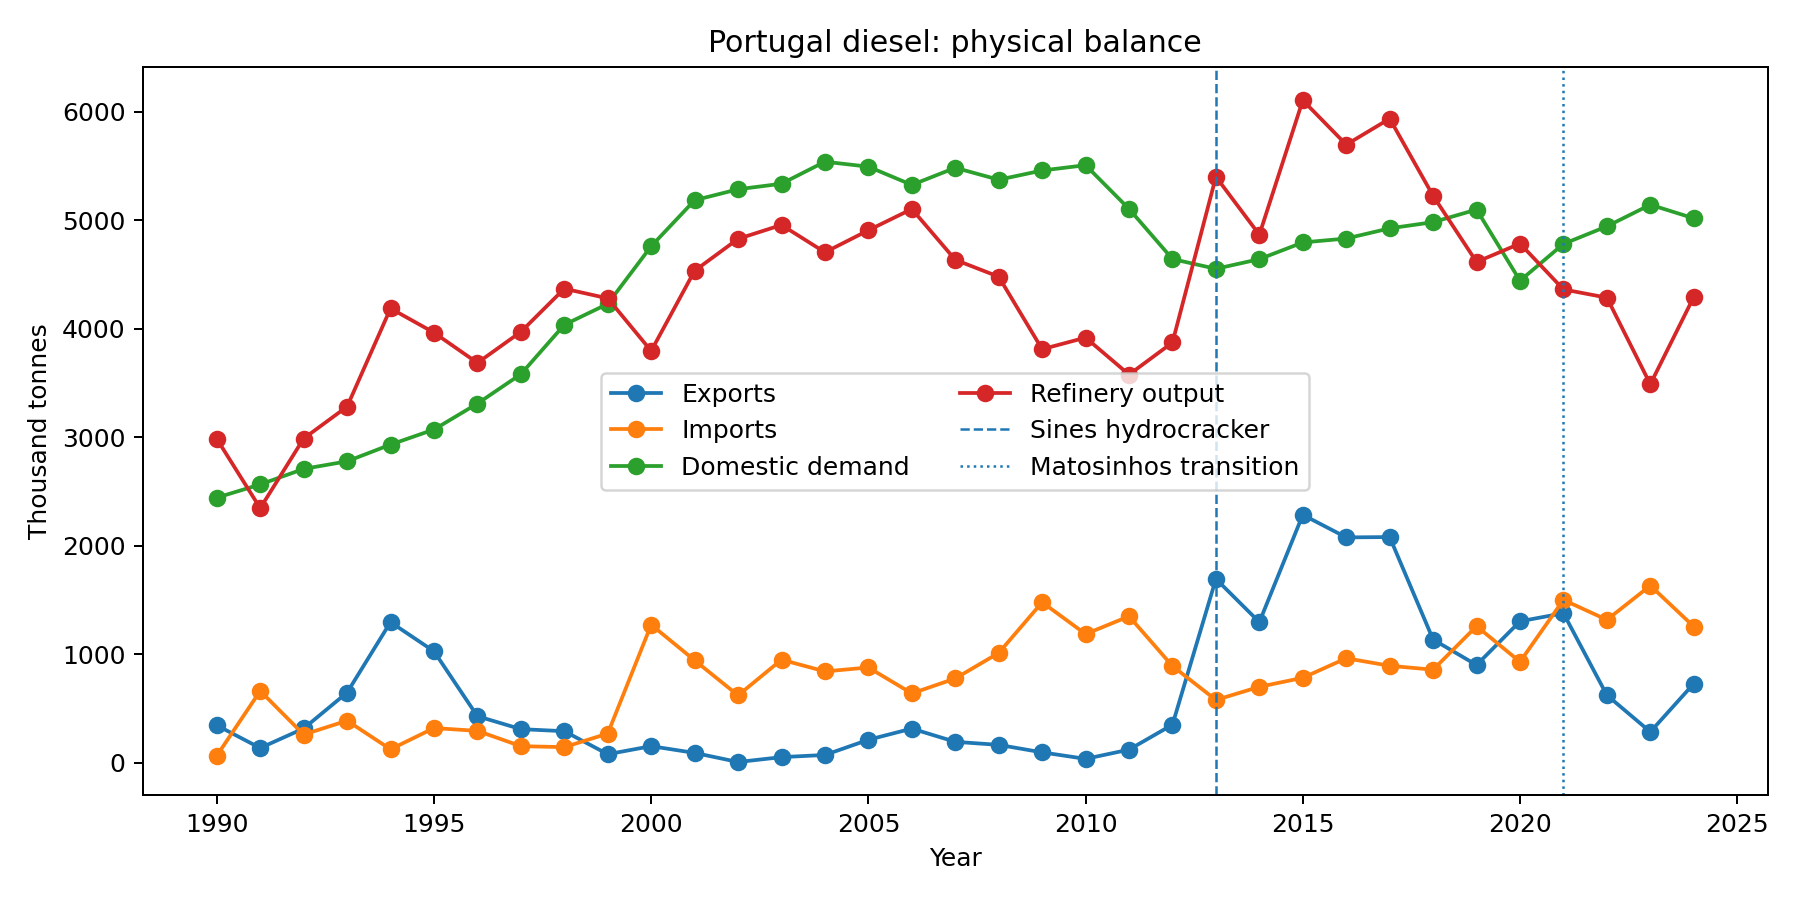
\includegraphics[width=0.92\linewidth]{diesel_physical_balance.png}
\caption{Portuguese diesel imports, exports, refinery output and demand, 1990--2024.}
\label{fig:dieselbalance}
\end{figure}

Diesel passes through the four regimes described in Section~\ref{sec:intro}. The line that
matters is the refinery-output-to-demand ratio crossing one, because a ratio above one means
the country manufactures more diesel than it burns and must place the surplus abroad, while a
ratio below one means the shortfall has to be bought.

Taking the later part of the window, from 2005 to 2012 Portugal is a net diesel importer with
output covering $0.70$ to $0.96$ of demand, so the gap was closed by imports in every one of
those years. From 2013 the ratio exceeds one and the net-import-to-demand ratio turns
negative, which is one event seen from the two sides of the same balance. From 2021 the system
returns to net import dependence, and by 2023 output covers only $0.678$ of demand, leaving
roughly a third of consumption to be sourced abroad.

Gasoline behaves differently. Portugal is a net gasoline exporter in every year of the window
except 1993, when imports briefly exceeded exports and the net-import-to-demand ratio reached $+0.06$.
Output covers between $0.94$ and $2.66$ times domestic demand, the low point being that same
year, and from 1994 onward the ratio never falls below one. The ratio rises after 2013 and
drifts down after 2021 without approaching one again, so there is no regime change comparable
to diesel's.

This is precisely the asymmetry the ratio definition warns about. A system can manufacture a
large surplus of one light product while importing another, and reading the output ratio as
self-sufficiency would obscure that. It also means the two products cannot be pooled, because an
aggregate petroleum-product dependence measure for Portugal would average a structural
exporter against a structural importer and describe neither.

\begin{figure}[htbp]
\centering
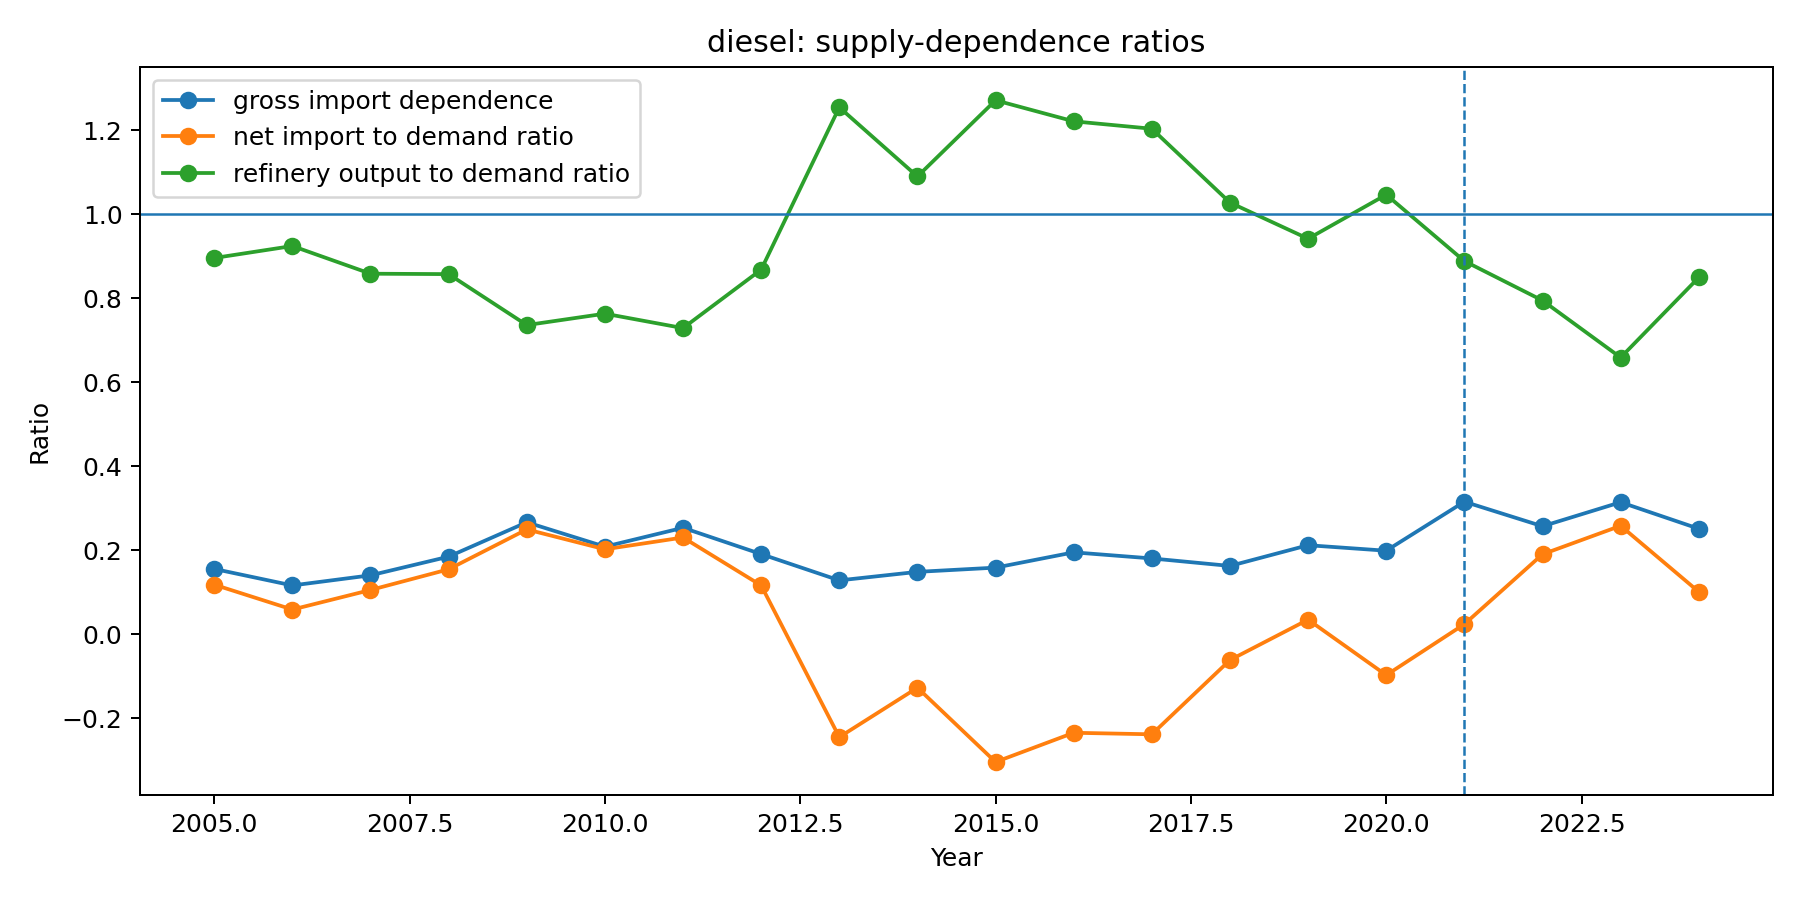
\includegraphics[width=0.92\linewidth]{diesel_dependence_ratios.png}
\caption{Diesel gross import dependence, net imports to demand, and refinery output to demand.
The output ratio crossing one in 2013 and falling back after 2021 is the central physical result
of this paper.}
\label{fig:dieselratios}
\end{figure}

\begin{table}[htbp]
\centering
\caption{Balance at the event years. The two independent trade sources disagree on the 2022
diesel export cell. The table carries the national figure of $622.2$~kt, which puts net imports
over demand at $+0.140$; the monthly source reports $331.0$~kt, which would put it at $+0.199$. Both values are carried through the supplementary
source-sensitivity tables.}
\label{tab:headline}
\small
\begin{tabular}{rlrrrrrl}
\toprule
Year & Product & Exports & Imports & Demand & Ref.\ out. & Net imp./dem. & Regime \\
\midrule
2012 & diesel & 350 & 890 & 4{,}641 & 3{,}872 & $+$0.116 & two refineries \\
2013 & diesel & 1{,}693 & 578 & 4{,}551 & 5{,}399 & $-$0.245 & two refineries \\
2020 & diesel & 1{,}303 & 929 & 4{,}441 & 4{,}783 & $-$0.084 & two refineries \\
2021 & diesel & 1{,}377 & 1{,}500 & 4{,}780 & 4{,}361 & $+$0.026 & transition \\
2022 & diesel & 622 & 1{,}316 & 4{,}942 & 4{,}285 & $+$0.140 & Sines only \\
2023 & diesel & 284 & 1{,}632 & 5{,}142 & 3{,}487 & $+$0.262 & Sines only \\
2024 & diesel & 728 & 1{,}254 & 5{,}017 & 4{,}291 & $+$0.105 & Sines only \\
\midrule
2012 & gasoline & 898 & 160 & 1{,}127 & 1{,}864 & $-$0.655 & two refineries \\
2013 & gasoline & 1{,}293 & 102 & 1{,}100 & 2{,}338 & $-$1.083 & two refineries \\
2020 & gasoline & 1{,}271 & 193 & 883 & 1{,}956 & $-$1.221 & two refineries \\
2021 & gasoline & 1{,}424 & 202 & 976 & 2{,}146 & $-$1.252 & transition \\
2022 & gasoline & 1{,}502 & 230 & 1{,}073 & 2{,}247 & $-$1.185 & Sines only \\
2023 & gasoline & 1{,}254 & 347 & 1{,}193 & 2{,}063 & $-$0.761 & Sines only \\
2024 & gasoline & 1{,}728 & 300 & 1{,}260 & 2{,}660 & $-$1.134 & Sines only \\
\bottomrule
\end{tabular}
\end{table}

\subsection{Structural breaks and event timing}

\begin{table}[htbp]
\centering
\caption{Chow tests at candidate break years, 2021 excluded as a transition year. 2013 and 2022
were pre-specified; 2000 was added after the panel was extended back to 1990 and is exploratory.}
\label{tab:breaks}
\begin{tabular}{llrrrrr}
\toprule
Product & Outcome & Break & $F$ & $p$ & BH $p$ & $n_{\text{pre}}/n_{\text{post}}$ \\
\midrule
gasoline & refinery output & 2000 & 22.00 & $<0.001$ & $<0.001$ & 10/13 \\
diesel & exports & 2013 & 21.58 & $<0.001$ & $<0.001$ & 13/8 \\
diesel & net imports / demand & 2013 & 21.40 & $<0.001$ & $<0.001$ & 13/8 \\
diesel & refinery output & 2000 & 11.68 & $<0.001$ & 0.0030 & 10/13 \\
diesel & refinery output & 2013 & 8.23 & 0.0032 & 0.0152 & 13/8 \\
diesel & imports & 2000 & 5.81 & 0.0108 & 0.0431 & 10/13 \\
\bottomrule
\end{tabular}
\end{table}

A Chow test asks whether one linear trend describes a series across a candidate year or whether
two fitted separately describe it better, so a rejection is a claim about the shape of the
series rather than about its level. It says the relationship generating the data changed, not
merely that the numbers moved.

Twenty-four tests are run across three candidate break years and six survive
Benjamini--Hochberg adjustment, but which series reject matters more than how many. Around 2000
the rejections are confined to refinery output, most strongly for gasoline ($F=22.0$, adjusted
$p<0.001$), and neither dependence ratio rejects. Output and demand rose together, so the
system grew without its trade position moving. A capacity expansion that keeps pace with
consumption is invisible to a dependence measure by construction, which is why 2000 is an
event in the production series and a non-event in the ratios.

At 2013 the pattern inverts. The rejections reach diesel exports and the net-import-to-demand
ratio, both at adjusted $p<0.001$, and refinery output rejects with them. That combination is
what separates the two years. A break in output alone is a statement about what the refineries
could make, whereas a break in the ratio is a statement about what the country had to buy, and
2013 is the only candidate year where both move together.

\begin{table}[htbp]
\centering
\caption{Interrupted-trend models, annual series, HAC(1), $n=34$, 2021 excluded. The 2022 export
rows depend on trade cells the two sources dispute, one for each product; the
supplementary material re-estimates them on each source. $^{\S}$This row holds the 2013 break constant; the row above fits 2022 alone, and the difference between them is why the annual evidence for a 2022 export break is weak.}
\label{tab:its}
\begin{tabular}{llrrrr}
\toprule
& & \multicolumn{2}{c}{Level change} & \multicolumn{2}{c}{Slope change} \\
\cmidrule(lr){3-4}\cmidrule(lr){5-6}
Product & Outcome, event & Estimate & $p$ & Estimate & $p$ \\
\midrule
diesel & exports, 2013 & $+$2{,}005.5 & $<0.001$ & $-$117.1 & $<0.001$ \\
diesel & exports, 2022 & $-$781.7 & 0.022 & $+$15.0 & 0.872 \\
diesel & exports, 2022$^{\S}$ & $-$570.0 & 0.078 & $+$150.1 & 0.166 \\
diesel & net imp./dem., 2013 & $-$0.540 & $<0.001$ & $+$0.029 & $<0.001$ \\
diesel & net imp./dem., 2022 & $+$0.201 & 0.031 & $-$0.017 & 0.616 \\
gasoline & exports, 2013 & $+$411.1 & 0.039 & $-$22.4 & 0.355 \\
gasoline & exports, 2022 & $-$270.9 & 0.121 & $+$69.3 & 0.413 \\
gasoline & net imp./dem., 2013 & $-$0.713 & $<0.001$ & $+$0.038 & 0.157 \\
gasoline & net imp./dem., 2022 & $+$0.307 & 0.095 & $+$0.070 & 0.457 \\
\bottomrule
\end{tabular}
\end{table}

The two annual designs disagree about 2022, and the disagreement is diagnostic. Chow tests
detect nothing on three post-event observations, which is a power statement rather than a null
result. The interrupted-trend model, which retains the whole series, detects a level shift in
diesel exports of $-782$~kt ($p=0.022$). That estimate is considerably weaker on the long series
than on a window beginning in 2005, and the gasoline estimates lose significance altogether, so
the annual evidence for 2022 is thinner than a short window suggests.

The monthly panel is partitioned into four phases: before May 2021, the Matosinhos transition
from May 2021 to February 2022, the energy-stress period from March 2022 to December 2022, and
post-stress from January 2023.

\begin{table}[htbp]
\centering
\caption{Diesel monthly means by event phase, kt per month unless noted.}
\label{tab:phases}
\begin{tabular}{lrrrrr}
\toprule
Phase & Months & Imports & Exports & Ref.\ out. & Net imp./dem. \\
\midrule
Pre-closure & 232 & 75.4 & 65.4 & 411.5 & 0.013 \\
Matosinhos transition & 10 & 133.3 & 63.0 & 321.9 & 0.162 \\
Energy stress 2022 & 10 & 111.1 & 27.7 & 324.6 & 0.193 \\
Post-stress & 24 & 117.5 & 42.3 & 311.7 & 0.181 \\
\bottomrule
\end{tabular}
\end{table}

Mean monthly diesel imports rise by roughly a half to three quarters between the pre-closure
phase and every subsequent phase, refinery output falls by about a fifth in the transition and
the stress phase and by nearly a quarter after, and the net-import-to-demand ratio moves from
approximately zero to $0.18$.

Two features of that pattern matter more than the individual figures. The three terms move in
the directions a capacity loss would produce, with imports up, output down and the balance
swinging from roughly even to buying about a fifth of consumption abroad. And no phase
recovers the pre-closure position, so what the means describe is a level change rather than a
disturbance the system worked through. These are raw averages that take no account of
seasonality or trend, which the model below does, and a seasonal pattern alone could produce
part of a phase difference this size.

\begin{table}[htbp]
\centering
\caption{Segmented monthly event model, diesel, $n=276$ months (2002--2024), month fixed
effects, HAC(3).
A phase coefficient is the level shift at that phase boundary against the extrapolated
pre-closure trend.}
\label{tab:monthly}
\small
\begin{tabular}{llrrrr}
\toprule
& & \multicolumn{2}{c}{No 2013 term} & \multicolumn{2}{c}{2013 held constant} \\
\cmidrule(lr){3-4}\cmidrule(lr){5-6}
Outcome & Term & Estimate & $p$ & Estimate & $p$ \\
\midrule
Refinery output (kt/month) & 2013 control & --- & --- & $+$167.92 & $<0.001$ \\
 & Matosinhos transition & $-$102.89 & 0.005 & $-$70.52 & 0.084 \\
 & Energy stress 2022 & $-$148.25 & $<0.001$ & $-$101.10 & $<0.001$ \\
 & Post-stress & $-$168.45 & $<0.001$ & $-$110.52 & 0.001 \\
 & \quad phase trend & $+$2.72 & 0.022 & $+$3.67 & 0.004 \\
\midrule
Imports (kt/month) & 2013 control & --- & --- & $-$47.65 & $<0.001$ \\
 & Matosinhos transition & $+$40.34 & 0.081 & $+$33.80 & 0.154 \\
 & Energy stress 2022 & $+$25.43 & 0.015 & $+$15.08 & 0.188 \\
 & Post-stress & $+$56.74 & $<0.001$ & $+$43.81 & 0.008 \\
\midrule
Net imports / demand & 2013 control & --- & --- & $-$0.4379 & $<0.001$ \\
 & Matosinhos transition & $+$0.1923 & 0.007 & $+$0.0878 & 0.307 \\
 & Energy stress 2022 & $+$0.3658 & $<0.001$ & $+$0.2198 & 0.005 \\
 & Post-stress & $+$0.4951 & $<0.001$ & $+$0.3174 & 0.001 \\
 & \quad phase trend & $-$0.0057 & 0.097 & $-$0.0086 & 0.020 \\
\midrule
\multicolumn{2}{l}{Adjusted $R^2$, refinery output} & 0.2163 & & 0.4046 & \\
\multicolumn{2}{l}{Adjusted $R^2$, net imports / demand} & 0.2931 & & 0.4982 & \\
\bottomrule
\end{tabular}
\end{table}

The monthly panel opens in 2002, so the 2013 hydrocracker sits inside it and the pre-closure
trend each phase is measured against was fitted through a step of $+167.92$~kt per month in
refinery output. Table~\ref{tab:monthly} reports both fits, and holding that step constant
raises the adjusted $R^2$ from $0.2163$ to $0.4046$ on output and from $0.2931$ to $0.4982$ on
the ratio. I read the results off the corrected column.

Each phase is measured against the same counterfactual, the pre-closure trend extrapolated
forward, never against the phase before it, so the coefficients do not add. On the corrected
fit, diesel refinery output sits $-101.10$~kt per month below that counterfactual during the
2022 stress phase and $-110.52$~kt below it from January 2023, with the net-import-to-demand
ratio $0.2198$ and $0.3174$ above it. What does not survive the correction is the Matosinhos
transition, at $-70.52$ ($p=0.084$) on output and $+0.0878$ ($p=0.307$) on the ratio. The
monthly design therefore identifies the 2022 stress and the level that followed clearly, and the
ten-month transition only weakly. The import rows weaken the same way, the energy-stress term
falling from $+25.43$ ($p=0.015$) to $+15.08$ ($p=0.188$), so I do not rely on the import channel
for either event.

The post-stress phase carries the evidence on whether 2023 was a trough or a level. Its terms
are large and firmly estimated, so 2023--2024 does not return to the pre-closure counterfactual,
while its phase trends run back towards it at $+3.67$~kt per month ($p=0.004$) on output and
$-0.0086$ ($p=0.020$) on the ratio. The system is displaced and recovering within the
displacement.

\subsection{The 2022 episode}

The chain tested here runs as follows. Russia supplied a large share of the world's vacuum gas
oil, which is a feedstock in diesel manufacturing at Sines, and Galp announced the suspension of
Russian oil-product purchases in March 2022 \citep{galprussian}. If that disruption bound, diesel
manufacturing should fall while gasoline manufacturing does not, because the constraint is on a
diesel feedstock and not on running the plant. Domestic demand still has to be met, so exports
should give way first and imports rise second. And because Portugal had been a one-refinery
system for ten months, none of that adjustment can be taken up domestically.

Each link holds in direction. Against a 2013--2019 baseline, 2022 diesel exports sit at the
zeroth percentile, diesel imports of $1{,}316$~kt sit $2.10$ standard deviations above the mean,
and diesel refinery output sits at $z=-2.04$. Gasoline exports are unremarkable at $z=-0.18$ and
gasoline refinery output is low but well inside its range at $z=-0.76$. Diesel demand is close to
its baseline mean at $z=0.58$, so the import surge is not demand-driven.

None of those scores places 2022, and the reason is the baseline rather than the statistic. A
score against a level mean measures the baseline trend whenever the baseline has one, and these
baselines trend: diesel imports rise across 2013--2019 at $88.05$~kt a year at $t=4.11$, and
diesel demand at $t=16.83$. Correcting for that means extrapolating a 2013--2019 trend across
2020 and 2021, which is not credible for any of these series; done for demand it puts 2022
roughly fifteen residual standard deviations below expectation. The median-and-MAD form does not
help, because it is robustness to spread and the defect is trend. The prediction interval the
baseline supports for diesel imports runs from $295$ to $1{,}427$~kt and contains $1{,}316$, as
it does for exports, net imports and refinery output. A percentile of zero or of one hundred out
of seven observations is a statement about seven numbers.

This section therefore describes the 2022 episode and does not carry it. The instrument for 2022
is the monthly segmented model, which fits a trend and measures each phase against its
extrapolation. What the balance shows is that its four terms move together in the pattern a
feedstock constraint implies, and that pattern is the argument.

Read as a whole, the four terms of the balance identify where the constraint bound. Refinery
output falls to the bottom of its baseline range while gasoline output does not, which locates
the problem in diesel manufacturing rather than in running the refinery. Demand sits at its
baseline, so nothing was rationed. Exports collapse and imports reach the top of the baseline
range. A system that cannot make as much of a product, and whose consumers want the usual amount
of it, has two ways to close the gap: stop selling it abroad and start buying it. Portugal did
both.

This is what the trade channel absorbing a shock looks like, and it is the only direct
observation in this paper of resilience in the sense of Section~\ref{sec:design} being tested.
The domestic buffer contributed nothing, since output moved the wrong way, which is what a
feedstock disruption does. Whether that counts as a system coping or a system exposed depends on
the terms on which those imports were obtained, which are not in the data.

2022 diesel exports is also the single largest disagreement between the two independent trade
sources, and the reconciliation identifies the monthly source as the outlier for that cell. The
qualitative result is unchanged on either value, since every baseline year exceeds both, but the
magnitude is not. The standardised deviation is $-2.44$ on the monthly source and $-1.89$ on the
corroborated national figure. The weaker of the two is the one I rely on.

\subsection{Portugal against Spain}

\begin{table}[htbp]
\centering
\caption{Diesel balance ratios, Portugal against Spain.}
\label{tab:spain}
\begin{tabular}{rrrrrrr}
\toprule
& \multicolumn{3}{c}{Refinery output / demand} & \multicolumn{3}{c}{Net imports / demand} \\
\cmidrule(lr){2-4}\cmidrule(lr){5-7}
Year & PT & ES & PT$-$ES & PT & ES & PT$-$ES \\
\midrule
2018 & 1.049 & 0.899 & $+$0.150 & $-$0.056 & $-$0.046 & $-$0.010 \\
2019 & 0.905 & 0.902 & $+$0.003 & $+$0.070 & $-$0.032 & $+$0.102 \\
2020 & 1.077 & 0.932 & $+$0.145 & $-$0.084 & $-$0.051 & $-$0.033 \\
2021 & 0.912 & 0.847 & $+$0.065 & $+$0.026 & $+$0.009 & $+$0.016 \\
2022 & 0.867 & 0.904 & $-$0.037 & $+$0.140 & $+$0.001 & $+$0.139 \\
2023 & 0.678 & 0.923 & $-$0.245 & $+$0.262 & $-$0.041 & $+$0.303 \\
2024 & 0.855 & 0.898 & $-$0.043 & $+$0.105 & $-$0.040 & $+$0.145 \\
\bottomrule
\end{tabular}
\end{table}

Spain refines the same products, shares a long border across which fuel moves in response to
price and tax differences \citep{leal2009prices, banfi2005fuel, teixido2024carbon}, and shares a
product market, and faced the same
withdrawal from Russian products on the same timetable. What differs is the event: Portugal
closed a refinery in May 2021 and Spain did not. If the post-2021 Portuguese movement were the
European shock working through any Iberian refining system, Spain should show something like it.

Over 2018--2024 Spanish diesel output covers between $0.85$ and $0.93$ of Spanish demand with no
trend over those years, and Spanish net imports stay within $0.052$ of balance. Portugal covered
more of its own diesel demand than Spain did in 2018, 2020 and 2021, and less from 2022, falling
to $0.678$ in 2023 while Spain sat at $0.923$. Portugal reaches $0.262$ on the net-import-to-demand
ratio in the same year. The comparison is confined to those years deliberately, because across the full panel
the Spanish ratio is not flat either, falling to $0.667$ in 2007 before recovering, so a claim of
stability is defensible only over the window shown.

Spain is a comparison series, not a control. A control would have to be alike in every relevant
respect except the treatment, and two national refining sectors never are. Crude slate, refinery
maintenance schedules, inventory positions and demand composition all differ, and the VGO
disruption did not fall on the two countries equally.

\subsection{Prices}

The order of these tests is not arbitrary, because each one licenses a different model. A
series with a unit root wanders without returning to a fixed level, and regressing one such
series on another produces a strong-looking relationship whether or not any relationship
exists. The first question is therefore whether the price levels are stationary, since a plain
regression is only safe if they are. If they are not, the second question is whether the two
wander together, which is what cointegration means and what makes an error-correction model
the right form.

Augmented Dickey--Fuller tests \citep{dickey1979distribution, said1984testing} on the log
levels do not reject a unit root for diesel in either
country, at $p=0.123$ for Portugal and $p=0.119$ for Spain. For gasoline they reject
marginally, at $p=0.019$ and $p=0.028$, and that verdict is not quite robust: of the six
combinations of deterministic term and lag rule tried per series, the Spanish one fails to reject
in the case with a trend and lags by BIC, at $p=0.074$. Across all of them, no series rejects at
one per cent. Neither product, then, clears the bar for a levels regression.

Both pairs are cointegrated in logs \citep{engle1987cointegration}, diesel at $p<0.001$ and
gasoline at $p=0.0026$. The two
results together settle the specification for both products: the levels wander, they wander
together, and an error-correction model is what fits a pair that behaves that way.

\subsubsection*{The levels model, and why it is not used}
\label{sec:levels}

The levels regression was estimated and is retained in the supplementary material, flagged as
not valid for inference for both products. It is reported because discarding it silently would
hide how much specification choice matters. On that specification the diesel interaction term
$\text{ES}\times\text{post}$ is $-0.082$ ($p<0.001$), which says that Portuguese prices became
\emph{less} responsive to Spanish prices after the transition. The licensed error-correction
model gives $+0.662$ ($p<0.001$) on the same interaction, the opposite sign. The levels model
also reports a deterministic trend of $-0.015$ per week ($p=0.005$). Both features are what a
regression between two integrated series estimated without its cointegrating relationship is
expected to produce, and the sign reversal is why the stationarity bar is set at one per cent
rather than five.

\begin{table}[htbp]
\centering
\caption{Error-correction models, two-step Engle--Granger, HAC(8), $n=993$ weeks.}
\label{tab:ecm}
\begin{tabular}{llrrr}
\toprule
Product & Term & Estimate & Std.\ error & $p$ \\
\midrule
diesel & Disequilibrium (lagged) & $-$0.1415 & 0.0266 & $<0.001$ \\
 & \quad $\times$ post & $-$0.4580 & 0.0845 & $<0.001$ \\
 & \quad post-period level & $-$0.5995 & 0.0802 & $<0.001$ \\
 & $\Delta \log$ ES & 0.7129 & 0.0397 & $<0.001$ \\
 & \quad $\times$ post & 0.6624 & 0.0946 & $<0.001$ \\
 & \quad post-period level & 1.3753 & 0.0859 & $<0.001$ \\
 & post & $-$0.0090 & 0.0021 & $<0.001$ \\
\midrule
gasoline & Disequilibrium (lagged) & $-$0.0911 & 0.0355 & 0.010 \\
 & \quad $\times$ post & $-$0.2767 & 0.0859 & 0.001 \\
 & \quad post-period level & $-$0.3678 & 0.0782 & $<0.001$ \\
 & $\Delta \log$ ES & 0.7891 & 0.0719 & $<0.001$ \\
 & \quad $\times$ post & 0.2846 & 0.2356 & 0.227 \\
 & \quad post-period level & 1.0738 & 0.2244 & $<0.001$ \\
 & post & $-$0.0029 & 0.0017 & 0.092 \\
\bottomrule
\end{tabular}
\end{table}

Both long-run relations are close to unit elastic:
$\log \text{PT} = 0.193 + 0.970 \log \text{ES}$ for diesel and
$\log \text{PT} = 0.123 + 0.978 \log \text{ES}$ for gasoline. The adjustment speed, the share of
a gap against that relation closed each week, more than quadruples for both products on that
specification after the
transition. For diesel it moves from $-0.142$ to $-0.600$, shortening the half-life of a
deviation from $4.5$ to $0.8$ weeks. For gasoline it moves from $-0.091$ to $-0.368$, a
half-life of $7.3$ weeks falling to $1.5$. Both are precisely estimated on that specification.

That specification holds the cointegrating vector fixed across the sample while letting the
adjustment speed break, and a regime-shift search puts a break in the vector itself at 2013,
eight years earlier. Whatever part of that shift is unmodelled sits in the disequilibrium term,
where the post-2021 interaction can absorb it. Refitting to allow the shift separates the
products: the diesel interaction holds at $-0.4055$ ($p<0.001$), a speed ratio of $2.9648$,
while the gasoline interaction falls to $-0.1878$ on an interval of $[-0.388, 0.013]$ with
$p=0.0664$. The contemporaneous elasticities move by less than a hundredth under the same
refit. Tested as one hypothesis rather than three, the separation is starker: the joint restriction
that the transition changed nothing in level, pass-through or adjustment gives $F=24.3169$ for
diesel and $F=1.3365$ for gasoline under the corrected specification, at $p<0.001$ and
$p=0.2611$. I carry the diesel result forward and treat the gasoline adjustment change as not
established.

The two products differ in the other channel. The diesel contemporaneous elasticity rises from
$0.713$ to $1.375$, precisely estimated ($p<0.001$). The gasoline contemporaneous elasticity does
not move on that specification, its interaction being $0.285$ with $p=0.227$. That result does
not survive a second break. Tested jointly, a March 2022 regime is rejected for diesel
($p=0.223$) but accepted for gasoline ($p=0.020$), and split at both dates the gasoline
elasticity runs $0.789$ before the closure, $1.679$ during the transition and $1.051$
afterwards. Gasoline's elasticity is therefore not permanently higher, which is a narrower
claim than that it never moved.

\begin{figure}[htbp]
\centering
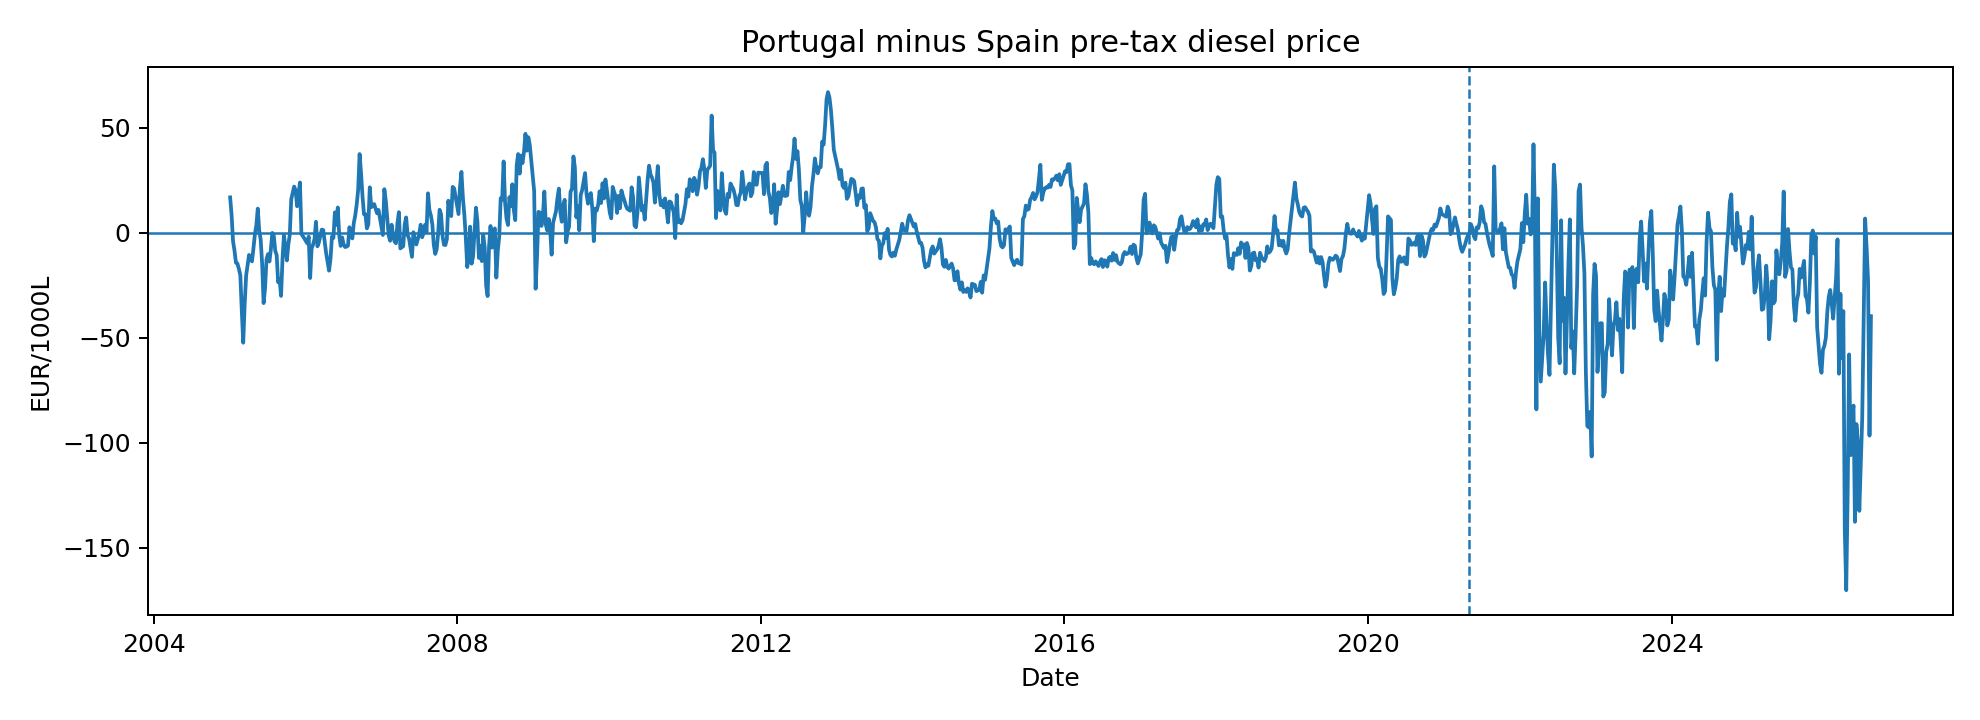
\includegraphics[width=0.49\linewidth]{pt_es_diesel_pretax_price_spread.png}
\hfill
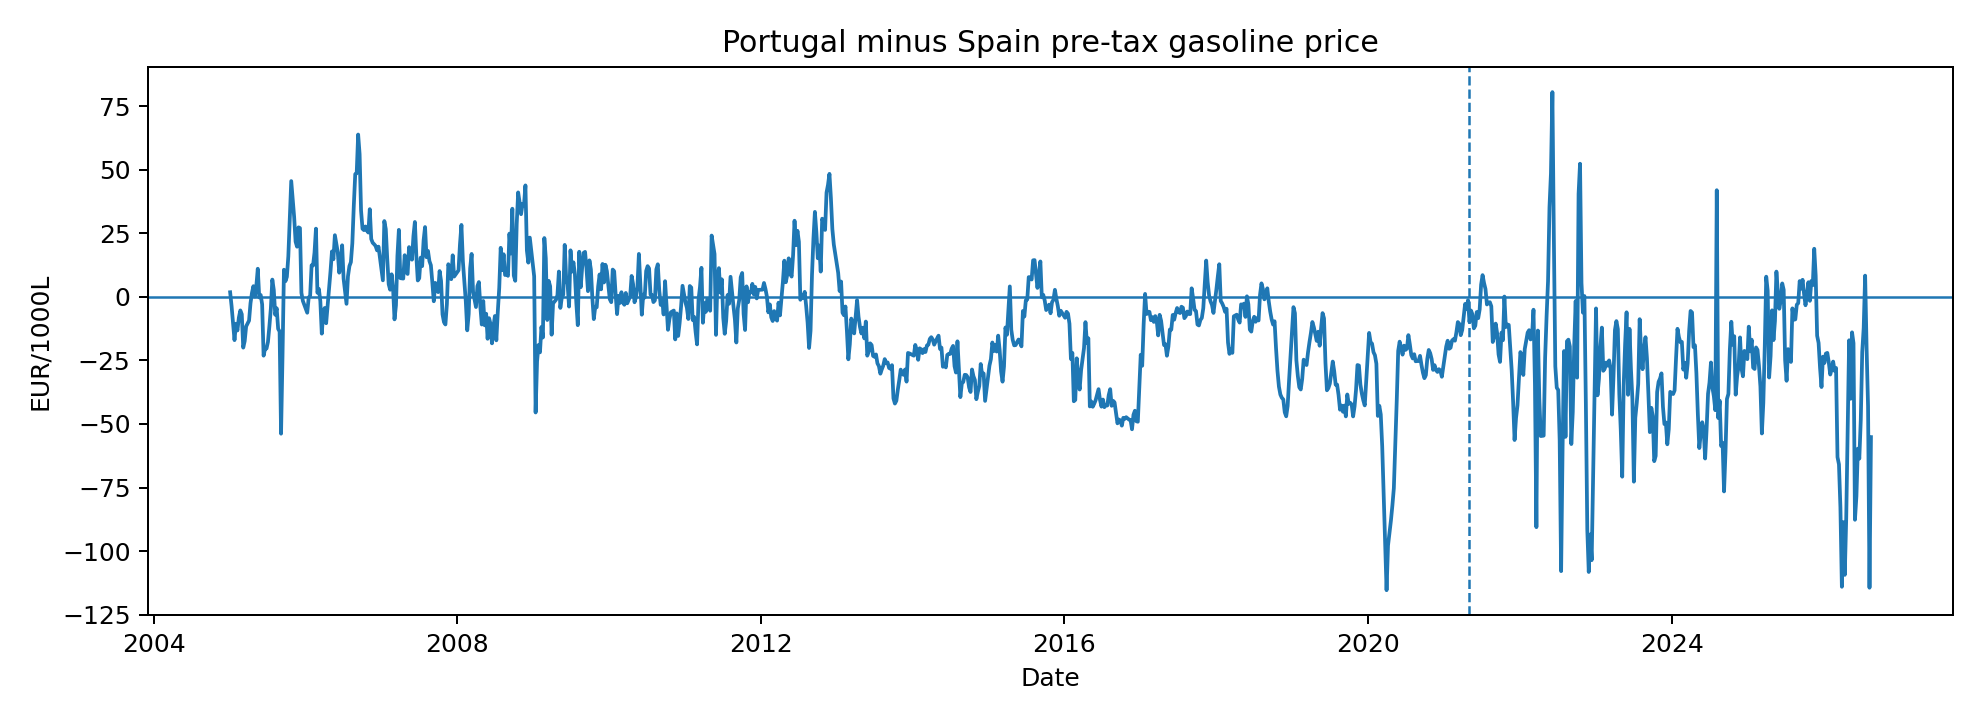
\includegraphics[width=0.49\linewidth]{pt_es_gasoline_pretax_price_spread.png}
\caption{Portugal and Spain weekly pre-tax prices and their spread: diesel (left),
gasoline (right).}
\label{fig:spreads}
\end{figure}

The mean Portugal-minus-Spain pre-tax diesel spread moves from $+4.12$ to $-26.71$ EUR per
1000~litres across the transition, a change of $-30.83$. The gasoline spread moves by
$-18.90$. These are descriptive. Under test both spreads reject a unit root, on $994$
observations each, though not with the same confidence: the gasoline spread rejects decisively
(ADF $p=0.0017$) while the diesel spread clears five per cent and no more ($p=0.043$). Neither
result is a second opinion on the cointegration test, because the raw difference is the
cointegrating combination only at a unit coefficient in levels. The estimated slopes are
$0.970$ and $0.978$ and the relation is in logs, so the EUR spread and the modelled residual
need not behave alike.

The specification matters for the diesel figure. A difference-only model, which the diagnostics
do not licence and which the supplementary material reports, gives a materially lower post-transition
elasticity, because omitting the disequilibrium term loads part of the adjustment
onto the contemporaneous coefficient. That gap is why I select the model family from
diagnostics.

\subsection{Placebo tests}

Two objections to the price result are testable, because the bulletin prices every member state
on the same definition. If the disequilibrium term simply became more volatile after 2021, every
pair priced against Spain would show a faster adjustment speed at that date. An adjustment
speed is only defined against an equilibrium the pair has, and on diesel log levels the same
diagnostic that licenses an error-correction model for Portugal declines it for Italy
($p=0.4213$) and Germany ($p=0.0727$), so neither is relied on. Among the pairs it does license,
Portugal gives a ratio of $4.24$ ($p<0.001$) against France at $0.99$ ($p=0.990$) and Belgium at
$1.11$ ($p=0.624$). Comparing per-pair $p$-values against a threshold is itself an uncontrolled
family, so the licensed pairs are also stacked into one regression and the restriction that
every control interaction is zero is tested at once, clustered on the date. For diesel it does
not reject, at $F=0.2058$ and $p=0.8140$.

For gasoline it does. Three pairs are licensed there and the same restriction rejects at
$F=13.7185$ ($p<0.001$), with France and Germany both slowing at the same date. The gasoline
movement in May 2021 is not Portugal-specific, so that result fails the placebo as well as the
specification test of Section~\ref{sec:results}.

A single break at May 2021 attributes to that date everything after it, including the seaborne
crude embargo of 5 December 2022 \citep{eu2022embargo}, which falls on every member state at
once. Splitting the post-closure period at the embargo separates the two. Between the closure
and the embargo the Portuguese speed moves from $-0.1415$ to $-0.8294$ ($p<0.001$) and neither
licensed neighbour moves comparably. From the embargo onward the pattern reverses, Belgium
rising to $-0.6223$ with its embargo interaction at $p=0.028$. The movement among the
neighbours belongs to the embargo, and the Portuguese movement to the window that contains the
closure.

The second objection is that the date is arbitrary. Estimated on the pre-closure sample only, so
that they cannot recover a diluted version of the real effect, false breaks at May 2011, 2013,
2015, 2017 and 2019 give ratios of $0.25$, $0.34$, $0.60$, $1.12$ and $1.60$, the two
significant ones running the wrong way. The sequence is monotone in the date, so the two nearest
the closure are the weakest placebos and a tightening that began before May 2021 and accelerated
at it cannot be separated from a step.

\subsection{Robustness}

Three checks bound how much the results depend on choices made in setting them up.

\begin{table}[htbp]
\centering
\caption{Pre/post difference around 2021 by window, 2021 excluded.}
\label{tab:windows}
\begin{tabular}{llrrr}
\toprule
Product & Outcome & 3 pre / 2 post & 5 pre / 3 post & 8 pre / 3 post \\
\midrule
diesel & net imports / demand & $+$0.224 & $+$0.277 & $+$0.323 \\
diesel & refinery output / demand & $-$0.238 & $-$0.283 & $-$0.315 \\
gasoline & net imports / demand & $+$0.333 & $+$0.393 & $+$0.281 \\
gasoline & refinery output / demand & $-$0.388 & $-$0.424 & $-$0.321 \\
\bottomrule
\end{tabular}
\end{table}

The first varies the pre- and post-event windows around the 2021 transition. The direction of
every dependence measure is the same across all three windows and only the magnitudes move, so
the headline five-and-three window is not doing the work. On that window diesel gross import
dependence rises from $0.202$ to $0.278$, the net-import-to-demand ratio rises from $-0.108$ to
$0.169$, and the refinery-output-to-demand ratio falls from $1.083$ to $0.800$.

\begin{table}[htbp]
\centering
\caption{2022 interrupted-trend level changes, computed on each trade source.}
\label{tab:sourcesens}
\begin{tabular}{llrrrr}
\toprule
& & \multicolumn{2}{c}{Primary source} & \multicolumn{2}{c}{Corroborated} \\
\cmidrule(lr){3-4}\cmidrule(lr){5-6}
Product & Outcome & Estimate & $p$ & Estimate & $p$ \\
\midrule
diesel & exports & $-$781.7 & 0.022 & $-$781.7 & 0.022 \\
diesel & net imp./dem. & $+$0.201 & 0.031 & $+$0.201 & 0.031 \\
gasoline & exports & $-$270.9 & 0.121 & $-$202.8 & 0.149 \\
gasoline & net imp./dem. & $+$0.307 & 0.095 & $+$0.253 & 0.111 \\
\bottomrule
\end{tabular}
\end{table}

The second re-estimates every 2022 annual result on each of the two trade sources, since the
disputed cells fall in that year. One result changes significance, in that the 2022 gasoline
export shift does not reach five per cent under either source once the panel is extended, and it is
marked wherever it appears and relied on nowhere. The diesel results do not depend on the
disputed cell, because the annual panel uses the corroborated source throughout.

The third is multiplicity. Twenty-four Chow tests invite false positives, and a Benjamini--Hochberg
correction across all of them leaves six surviving. The 2013 diesel results survive
comfortably. The 2022 tests do not survive because they never reached significance to begin
with, which is a power statement about three post-event observations. A fourth check is
internal. The Eurostat panel permits a balance identity, $Q^{\text{refinery}} + M - X - D$, that
the four reported terms do not close. Across 1990--2024 the Spanish gasoline residual ranges
from $-20.0$ to $+15.2$ per cent of demand and the Spanish diesel residual from $-14.7$ to
$+13.9$. The Portuguese ones are smaller but still reach $-9.1$ and $+12.0$. Residuals of that
size reflect stock changes, refinery fuel and statistical differences, and they are the reason
nothing here infers stock behaviour from the balance, since a residual this large would swamp
any inventory signal it might carry.

\section{Discussion}
\label{sec:discussion}

\subsection{Why the two products diverge}

The two products behave differently in almost every result above, and the reason is visible in
the window means rather than in anything about how they were treated. Portugal consumes roughly
three times as much diesel as gasoline while manufacturing considerably more gasoline than it
consumes. Portuguese demand dieselised. Gasoline demand peaks in 2000 and no later year matches
it, while diesel demand peaks in 2004, and the gap between the two widened over the window.

A refinery's products come out of the same barrel in proportions bounded by its configuration, so
gasoline output is not an independent decision: cutting it means cutting throughput, and
cutting throughput means making less diesel too. A country running its plants at the rate its diesel
demand requires will produce more gasoline than it needs, and the surplus is exported because the
alternative is not producing the diesel. The persistent gasoline export surplus is therefore a
residue of running the system for diesel, not a strength in gasoline.

That difference in starting position governs the responses. A hydrocracker converts heavy gasoil
into middle distillates, so the 2013 unit acted on the deficit product, and diesel output
peaks at $6{,}104$~kt in 2015 as the trade position crosses into surplus, while gasoline had no deficit
to close and shows no comparable break. The same asymmetry governs the losses. Gasoline entered
the 2021 closure with output well above domestic demand, so removing capacity moved the ratio
down a wide margin without reaching one, and gasoline coverage stays above $1.7$ in every year
after the closure. Diesel entered with a ratio near one and no comparable margin, so the same
proportional loss pushed it to $0.678$ by 2023. A buffer is only protective while it is large
relative to the shock, and Portugal held a large one in the product it did not much need and a
thin one in the product it did.

This account is consistent with every result above but is not tested by any of them. Yield
economics, the crude slate and the commercial logic of export contracts are not observed here,
and a competing account resting on contracting rather than chemistry would fit the same series.

\subsection{What the closure changed beyond capacity}

The quantity that changed in May 2021 is capacity. But the closure also changed the shape of the
system in ways a capacity figure does not express, and those bear on how the 2022 shock was met.
What follows is structural reasoning about a documented event, not an estimate.

With two refineries, an interruption confined to one leaves the other running and the national
balance absorbs part of the loss internally. With one, an interruption has no domestic offset at
any price and the entire adjustment must run through trade. Turnarounds can be staggered across
two sites so that some conversion capacity is always available, and cannot across one. Two plants
of different configuration can be run to different slates. One plant's slate is set by its own
configuration and the crude available to it.

The consequence that matters most is the concentration of the feedstock exposure. The 2022
disruption was specific to vacuum gas oil, a diesel feedstock at Sines. Before May 2021 a
VGO-specific problem at Sines would have left Matosinhos unaffected. After it, Sines was the whole
of Portuguese refining, so a shock to one feedstock at one plant was a shock to national diesel
manufacturing. The closure concentrated the capacity and its feedstock vulnerability in the same place,
ten months before that vulnerability was tested. How a two-site system would have met the same
disruption is not estimated here.

\subsection{What can and cannot be inferred}

The causal question is open and this design cannot close it. The transition and the largest
European product-supply shock in decades fall ten months apart, too close for annual data and
close enough that the monthly design separates them only under an assumption about the shape of
the trend between them.

More than that, the two are not independent in a way a better estimator would fix. The closure
changed the structure through which the shock propagated, so asking how much of 2022 was the
shock and how much was the closure presumes a decomposition the physical system does not have.
On that reading the closure and the shock are not competing explanations. The closure determined
how a subsequent shock would propagate. The shock determined when that would be tested. Gasoline
is the nearest thing to a control the data supplies, having gone through the same closure at
the same plant while showing almost none of it in the physical balance, because it entered with
a margin diesel did not have. It is not a clean control: its price adjustment speed moved by
much the same factor as diesel's.

What follows for policy is correspondingly narrow. The structural exposure measures moved
together and in one direction, which a policy discussion would need to start from. But stocks,
storage, port capacity, supplier diversity and the terms on which the additional imports were
obtained are not observed, and those determine whether higher import exposure is a vulnerability
or simply a different and possibly cheaper way of meeting demand. A reader who takes rising
import dependence as \emph{prima facie} evidence of reduced security is going beyond what is
shown here.

The price finding carries the same limit in a different form. Portuguese pre-tax diesel prices
now track Spanish ones more closely and revert to the Iberian relation several
times faster, which amounts to a loss of domestic price insulation. That reading sits naturally
alongside the physical result, since a country meeting more of its diesel demand from imports is
buying at prices formed in the market those imports come from. But it is co-movement between two
retail series rather than pass-through, and the specification controls for nothing the two
markets have in common, and the same tightening would follow from a period in which common cost shocks came to
dominate both. Gasoline is the useful check, and it is the observation least favourable to the
framing here, since its adjustment speed moves by a similar factor while its physical position
barely changed. Nothing in this paper speaks to refinery-gate or wholesale prices, which are not
observed at all.

\subsection{Limitations}

Eleven limitations bound the results, in rough order of how much they matter.

\begin{enumerate}
\item \textbf{2022 confounds the post-closure window.} The transition and the European energy
shock fall ten months apart. The monthly model separates them statistically, but COVID-recovery
demand, Sines maintenance and the Russian VGO disruption are not separately identified. Two of
those run through the concentration the closure produced and are therefore not alternatives to
it. Unplanned maintenance is the one that is genuinely independent, and no series here rules it
out.
\item \textbf{No causal design.} No control group, instrument or counterfactual is used. Every
post-2021 result is an association measured around a documented event. The Spain comparison
constrains the common-shock explanation but does not license difference-in-differences, and no
pre-trend or common-shock diagnostics have been estimated.
\item \textbf{Low annual power after 2021.} Three post-event annual observations cannot support
a Chow test. The interrupted-trend models carry the annual evidence for 2022, and they impose a
common trend the Chow design does not.
\item \textbf{The post-transition period carries the whole price result.} Every interaction
in the error-correction models is identified off $190$ weeks, a fifth of the sample, and those
weeks contain the 2022 price episode. Re-estimating without 2022 and on each half of the
period leaves the direction intact and moves the multiple of the pre-transition adjustment
speed between $2.96$ and $4.40$.
\item \textbf{Generated regressor in both error-correction models.} The disequilibrium term is
estimated in a first stage, so second-stage standard errors are conditional on it
\citep{pagan1984econometric}. A single-step
or maximum-likelihood estimator would price that uncertainty properly. So does the assumption
that one cointegrating vector, estimated over the whole sample, holds on both sides of the
transition.
\item \textbf{Retail, not wholesale, prices.} The Weekly Oil Bulletin reports consumer prices.
The price results describe retail co-movement, not refinery-gate or international wholesale
transmission, and are not pass-through in the causal sense.
\item \textbf{DGEG trade covers only 2019--2024.} The 2013 break is corroborated against
Eurostat, which is compiled from the DGEG submission rather than independent of it.
\item \textbf{The gasoline price result fails two independent checks.} It does not survive
letting the cointegrating vector shift at 2013, and the licensed controls move jointly at the
same date. Neither on its own would be decisive; together they are why no gasoline adjustment
claim is made.
\item \textbf{One cointegrating vector across a break.} The long-run relation is estimated over
the whole sample while the adjustment speed is allowed to break, and the date a regime-shift
search selects for the relation itself is 2013 rather than 2021. Refitting with the relation
allowed to shift at that date is reported in the price results above: the diesel adjustment
change survives it and the gasoline change does not, at $p=0.0664$. The contemporaneous
elasticities are unaffected. This is the assumption that costs the paper a result, and it is
reported rather than relegated.
\item \textbf{The Spanish comparison is smaller than its own measurement error.} The Spanish
diesel balance residual reaches $15$ per cent of demand, against Spanish net imports staying
within $0.052$ of balance. Spanish flatness is therefore qualitative. The Portuguese movement,
about $0.40$ on the coverage ratio, is several times its residual and is not affected the same
way.
\item \textbf{Balance residuals are not closed.} The four Eurostat terms do not sum to zero and
stock changes are not modelled.
\item \textbf{JODI assessment codes unverified.} All Portuguese observations carry assessment
code 1, whose exact semantics have not been confirmed against JODI documentation.
\end{enumerate}

\subsection{What evidence would settle it}

Three post-closure annual observations cannot support a Chow test, and several results here are
weak precisely because the post-event window is short. A few more years would let the annual
designs speak, and would show whether the 2023 coverage figure was a trough or a level.

Three other kinds of evidence would do more than waiting. A monthly series of Sines throughput
and unplanned outages would separate a feedstock disruption from a maintenance event, which
annual balances cannot distinguish and which is the most troubling of the remaining alternatives.
An import-origin series would show whether the additional diesel came from the markets that set
the Spanish price, the mechanism the price result is consistent with but does not demonstrate.
And refinery-gate or wholesale quotations would let the price question be asked as pass-through
rather than as co-movement.

Failing those, the cleanest natural experiment would be a comparable single-refinery closure
elsewhere in Europe at a date not adjacent to a continent-wide supply shock. The identification
problem here is not a shortage of Portuguese data. It is that the two events fall ten months
apart, and no amount of Portuguese data will move them.

\section{Conclusion}
\label{sec:conclusion}

Over thirty-five years Portugal's diesel system crossed the same line three times and ended
further from self-coverage than it began. It was a net exporter through most of the 1990s, a net
importer for the fourteen years from 1999, an exporter again from 2013 after the hydrocracker
in every year but 2019, and an importer in every year since 2021. By 2023 domestic manufacturing covered $0.678$ of
diesel demand and the net-import-to-demand ratio stood at $0.262$. Those are the window's
extremes, but narrowly: 2009 reaches $0.2534$ and $0.6982$ on a system with two refineries, and
the gap is a fraction of the $0.1487$ standard deviation of the annual change in that ratio.
What distinguishes 2023 is that the level was reached on half the manufacturing base.

Measured against the four quantities defined in Section~\ref{sec:design}, all four
moved, and none moved back. The domestic buffer thinned, import exposure rose on both measures,
and manufacturing concentrated from two sites to one; those three run the same way for
resilience as defined here. Price integration tightened on both channels, which is a different
kind of fact: closer coupling to a larger market raises exposure to prices formed elsewhere and
can equally widen access during a domestic interruption. The physical results carry the
resilience reading; the price result measures external price exposure and is reported as that.

Gasoline crossed none of them, which is not the same as saying it did not move. On the annual
ratios it moves at least as far as diesel: across the 2021 closure its net-import-to-demand
ratio shifts by $+0.393$ against diesel's $+0.277$, and its refinery-output-to-demand ratio by
$-0.424$ against diesel's $-0.283$. Its price adjustment speed quadruples much as diesel's
does on the fixed-vector specification, though unlike diesel's it does not survive letting the
long-run relation shift at 2013. What separates them is where they started: gasoline entered every one of these events
manufacturing roughly twice its domestic demand and left still manufacturing well above it, so
a movement of that size crossed no threshold, while diesel entered with a ratio near one and
the same proportional loss carried it across. What determined exposure was not the size of the
movement but how much margin the product had before it began.

Three things follow that are not specific to Portugal. The first is that a product-level
balance is the right unit of analysis for this question. An aggregate petroleum-product
dependence measure would have averaged a structural exporter against a structural importer and
shown a system barely moving, when one of its two products crossed from surplus to the heaviest
deficit in thirty-five years. The second is that the margin a product holds before a shock,
rather than the size of the shock, is what determines whether capacity loss shows up as
exposure. The third is that a closure is not only a subtraction of capacity, because it changes
the structure through which later shocks propagate, which is why the closure and the 2022 episode
resist being weighed against each other.

What the analysis cannot say is how much of the post-2021 position is permanent. Coverage
recovers from $0.678$ in 2023 to $0.855$ in 2024, which is consistent with 2023 having been the
trough of an adjustment and equally consistent with a system that now runs closer to its import
channel and fluctuates around it. Distinguishing those needs years this panel does not yet
have.

\section*{Verification and reproducibility}
\label{sec:verification}
\addcontentsline{toc}{section}{Verification and reproducibility}

Every quantity in this paper is generated by a pipeline that writes a checksummed evidence
bundle, and the paper is checked against that bundle before it is built. Twelve checks run: each
table's printed values must reproduce from the file that table is declared to come from, stated
sample sizes must match the fitted models, quoted test statistics must reproduce from columns
holding that kind of statistic, no claim may quote a coefficient from a model family the
diagnostics did not select, no estimate from a superseded specification may be quoted without
naming the specification, no bundle artifact may cover years the study window excludes, and
every quantity carrying a unit must be written where the numeric checks can read it.

Two limits are worth stating, because the checks are easy to over-read. Reproducibility against
the whole bundle is close to vacuous for a ratio printed at two or three decimals. The
bundle holds hundreds of dense ratio series, and at four decimal places two of six deliberately wrong
values still match. Only source-scoped checks discriminate. And no check verifies a claim about a
\emph{sequence} of values as opposed to individual ones, which is the class of error that has
most often survived review here.

The analysis code, the derived tables behind every figure and table above, the supplementary
material referred to throughout, and a document recording the provenance of each input are
available in the project repository \citep{repository}.

\bibliography{references}

\end{document}
